\documentclass{article}
\usepackage{graphicx} % Required for inserting images
\usepackage{datetime} % Add this line to include the datetime package
\usepackage{amsmath}
\usepackage{amssymb}
\usepackage{amsthm}
\usepackage{tikz}
%\usepackage{hyperref}
\usepackage{xcolor} % Required for defining custom colors

\definecolor{darkblue}{rgb}{0.0, 0.0, 0.5} % Define a darker blue color

\usepackage[colorlinks=true, linkcolor=darkblue, urlcolor=darkblue, citecolor=darkblue]{hyperref} % Use the darker blue color

% Define theorem style
\theoremstyle{plain} % Bold title, italic body
\newtheorem{theorem}{Theorem}
\newtheorem{lemma}[theorem]{Lemma}
\newtheorem{corollary}[theorem]{Corollary}

\theoremstyle{definition} % Bold title, normal body
\newtheorem{definition}[theorem]{Definition}
\newtheorem{example}[theorem]{Example}

\title{First Isomorphism Theorem}
\author{Aaron Honculada}
\date{\monthname[\month] \the\year}

\begin{document}

\maketitle

\section{First Isomorphism Theorem}
\begin{theorem}
    Let $f: R \to S$ be a ring homomorphism, then the quotient ring $R / \ker f$ is isomorphic to the image of $f$, $\text{Im}(f)$, i.e.
    \[
        R / \ker f \cong \text{Im}(f)
    \]
    where:
    \begin{itemize}
        \item $\ker f$ is the kernel of $f$, i.e. $\ker f = \{ r \in R \mid f(r) = 0 \}$
        \item $\text{Im}(f)$ is the image of $f$, i.e. $\text{Im}(f) = \{ f(r) \mid r \in R \}$
    \end{itemize}
\end{theorem}

The map $\tilde{f}: R / \ker f \to \text{Im}(f)$ is given by $\tilde{f}(r + \ker f) = f(r)$.

\begin{figure}[h]
    \centering
    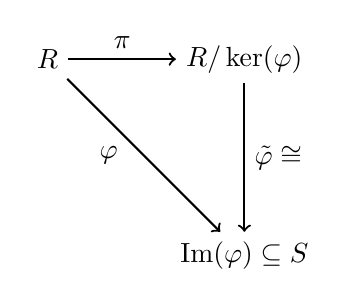
\begin{tikzpicture}[node distance=2.5cm, thick, ->]
        % Nodes
        \node (R) {$R$};
        \node (RmodK) [right of=R] {$R / \ker(\varphi)$};
        \node (S) [below of=RmodK] {$\operatorname{Im}(\varphi) \subseteq S$};

        % Arrows
        \draw[->] (R) to node[above] {$\pi$} (RmodK);
        \draw[->] (R) to node[left, xshift=-0.2cm] {$\varphi$} (S);
        \draw[->] (RmodK) to node[right] {$\tilde{\varphi} \cong$} (S);
\end{tikzpicture}
\caption{First Isomorphism Theorem}
\end{figure}

\begin{example}
    Let $\varphi: \mathbb{Z} \to \mathbb{Z}_6$ be the homomorphism defined by $\varphi(n) = n \pmod{6}$.
    Then the \textbf{kernel} of $\varphi$ is all integers that are mapped to 0 in $\mathbb{Z}_6$, meaning:
    \[
        \ker(\varphi) = \{ n \in \mathbb{Z} \mid \varphi(n) \equiv 0 \pmod{6} \} = 6\mathbb{Z}
    \]
    Since $6\mathbb{Z}$ is an \textbf{ideal} of $\mathbb{Z}$, we can consider the quotient ring:
    \[
        \mathbb{Z} / 6\mathbb{Z}
    \]
    The \textbf{image} of $\varphi$ consists of all values that $n \pmod{6}$ can take:
    \[
        \operatorname{Im}(\varphi) = \{ \varphi(n) \mid n \in \mathbb{Z} \} = \{ 0, 1, 2, 3, 4, 5 \} = \mathbb{Z}_6
    \]
    Therefore, by the First Isomorphism Theorem, $\mathbb{Z} / 6\mathbb{Z} \cong \mathbb{Z}_6$.
\end{example}


\end{document}